%
% Modelo LaTeX baseado no modelo A5L

% Nota: usar /newpage com 1 coluna
%       usar /clearpage com 2 colunas
%       o /newpage com duas colunas escreve na próxima coluna
\documentclass[a5paper,onecolumn, 11pt]{article}
\usepackage[landscape]{geometry}
\usepackage{indentfirst}
%Sample text
%\usepackage{lipsum}

%escrever acentos e coisas do género sem que o latex se desoriente
\usepackage[utf8]{inputenc}

%hifenização e titulos em portuguêsoa
\usepackage[portuguese]{babel}

%para ter a informação de quantas páginas tem o documento
\usepackage{lastpage}

%importar cores predefinidas
\usepackage[usenames,dvipsnames]{xcolor}
\definecolor{DarkGray}{gray}{0.40}

%usar multirow e multicolumn
\usepackage{multirow}

%para ter imagens, depois define a directoria de imagens
%\usepackage{graphicx}
\usepackage[pdftex]{graphicx}
\graphicspath{{imagens/}}

%poder ter texto sublinhado que passa para a linha seguinte automaticamente
%usar com \uline{my underline text}
\usepackage[normalem]{ulem}

%definir o cabeçalho e rodapé
\usepackage{fancyhdr}
\pagestyle{fancy}
\fancyhead[L]{
    \small{
        \textcolor{DarkGray}{
            \textbf{ProjectoCG}
        }
    }
}
\fancyhead[R]{
    \small{
        \textcolor{DarkGray}{
            \textbf{Pág. \thepage\ /\pageref{LastPage}}
        }
    }
}
\fancyfoot[C]{}

\begin{document}

\onecolumn
\thispagestyle{empty}
\begin{tabular}{ll}
    \multirow{7}{*}{ 
\includegraphics[height=90pt]{logo.jpeg} }
    &\\
    & \textcolor{DarkGray}{\Large{\textbf{Escola de Engenharia}}} \\
    &\\
    & \large{Departamento de Informática}\\
    &\\
    &\\
    & \large{Licenciatura em Engenharia Informática}\\
\end{tabular}
\begin{center}
    \Large{\textbf{Projecto de Computação Gráfica}}\\
    \vspace{20pt}
    \Large{\textbf{``Bar''}}\\
    \vspace{15pt}
    \begin{tabular}{r@{, }l}
        Bruno Ferreira&A61055\\
        Serafim Pinto&A61056\
    \end{tabular}
    
    \vspace{5pt}
    \emph{Grupo 19}\\\vspace{15pt}
    \large{\textbf{Braga, Maio de 2013}}
\end{center}

\newpage
\onecolumn
\tableofcontents
\newpage
\listoffigures

\newpage
\section{Resumo}
Neste relatório apresentamos todos os passos e decisões tomadas na construção do trabalho prático de Computação Gráfica.

Este projecto consiste na representação de um Bar, enquanto contrução geométrica. O Bar poderá conter elementos como mesas, cadeiras, copos, entre outros.

Numa primeira parte deste relatório fazemos uma breve introdução ao projecto, seguindo-se a análise do seu desenvolvimento ao longo das várias fases. Depois apresentamos uma descrição detalhada das técnicas usadas e, por fim, temos a conclusão.


\clearpage
\section{Introdução}
No desenvolvimento do presente projecto de Computação Gráfica pretendemos, para além de aplicar os conhecimentos leccionados na Unidade Curricular, desenvolver sensibilidade para a criação de aplicações de elevada complexidade gráfica. Propomos-nos portanto a criar um espaço com elementos comummente observados num Bar.

Este trabalho está dividido em quatro fases distintas. Na primeira fase apenas são feitas as primitivas: plano, cubo, cilindro, esfera. Numa segunda fase, devem ser apresentados alguns itens que deverão estar no espaço final, tais como: mesas, cadeiras, copos e candeeiros. A terceira fase consiste na preparação das primitivas das fases anteriores para a inclusão de texturas e iluminação. Nessa fase, devemos também optimizar o projecto utilizando \textit{Vertex Buffer Objects}. Na quarta e última fase deve ser montado o Bar propriamente dito, fazendo uso de tudo o que foi criado até ao momento. Além disto, a visualização do modelo deve ser feita recorrendo a uma câmara de movimento livre, com o uso do teclado e rato. Posto este problema, que está descrito no enunciado do trabalho, deveremos implementar e tornar possível a criação deste cenário seguindo os requisitos que serão apresentados no capítulo seguinte.

O projecto será desenvolvido em C++ no software Visual Studio 2012. Utilizaremos também a biblioteca gráfica do OpenGL, os utilitários GL (GLU) e o GL Extension Wrangler (GLEW).


\clearpage
\newpage
\section{Descrição do Trabalho e Análise de Resultados}
Neste capítulo vamos descrever o desenvolvimento de cada um dos requisitos a ser apresentados. Descreveremos também os principais passos da sua implementação e estruturação e faremos uma breve análise dos resultados obtidos com estas mesmas implementações.


\newpage
\onecolumn
\subsection{Requisitos}
Durante esta secção apresentamos em detalhe os requisitos propostos em cada fase para o desenvolvimento do nosso projecto.
\subsubsection{Primeira Fase}
\begin{itemize}
    \item{Construir uma biblioteca de primitivas: plano, cubo, cilindro e esfera;}
    \item{Cada primitiva deve ser feita numa função que desenhe a primitiva centrada na origem;}
    \item{A função para cada primitiva deve ter um conjunto de parâmetros que permita desenhar de acordo com a dimensão e resolução pretendidas;}
    \item{Construção de uma aplicação OpenGL que permita a visualização de cada primitiva separadamente.}
\end{itemize}
\newpage
\subsubsection{Segunda Fase}
\begin{itemize}
    \item{Apresentar rotinas que desenhem os seguintes objectos: mesas, cadeiras, copos e candeeiros;}
    \item{Desenhar o espaço limite do bar, ou seja, paredes chão e tecto;}
    \item{À exceção do copo, todos os outros objectos devem ser desenhados à custa da biblioteca de primitivas da primeira fase, e de transformações geométricas. O copo deve ter uma rotina própria para a sua construção;}
\end{itemize}
\subsubsection{Terceira Fase}
\begin{itemize}
    \item{Definição das coordenadas de textura e definição das normais nas primitivas;}
    \item{Utilização de VBOs;}
    \item{Construção de  uma aplicação que permita a visualização de cada composição geométrica.} 
\end{itemize}
\newpage
\subsubsection{Quarta Fase}
\begin{itemize}
    \item{Aplicação com a apresentação da composição geométrica final, ou seja, um bar com mesas, candeeiros, cadeiras e copos (construídos apenas com recurso às primitivas e transformações geométricas desenvolvidas nas fases anteriores);}
    \item{Utilização de texturas e iluminação.}
    \item{Visualização da cena utilizando uma câmara de movimento livre, sem necessidade de detecção de colisões.}
\end{itemize}
\newpage
\subsection{Implementação}
Nesta seccção descrevemos de forma incremental o desenvolvimento do projecto ao longo das 4 fases.
\subsubsection{Primeira Fase}
A  primeira fase  pedia que fosse construída uma biblioteca com primitivas  geométricas, aqui explicamos  como nesta fase do projecto construímos cada uma delas. Estas primitivas foram numa classe à qual chamámos \textbf{Primitivas}. Para facilitar a visualização destas, elaborámos também uma \textit{main.cpp}, onde é possível através do teclado mover a câmara e visualizar o objecto de ângulos diferentes.

Criámos também o módulo \textbf{Utilities}, onde temos pequenas funções que nos facilitam na escrita do código tornado-o mais fácil de ler (p.e função que passa de graus para radianos). Além disto, temos um menu associado ao botão direito do rato onde o utilizador pode escolher qual a primitiva a visualizar, e visualizar o objecto de várias formas (figura colorida, apenas linhas ou apenas pontos).
\newpage
\begin{description}
	\item[Plano] \hfill \\
	A função que desenha o plano recebe como argumentos, o comprimento, a largura e ainda o número de camadas que o plano terá. Como queremos o nosso plano com um determinado número de camadas, dividimos as variáveis comprimento e largura pelas camadas pretendidas,  e guardamos o resultado em \textit{x2} e \textit{z2} respectivamente (sobre camadas, ver secção \ref{Camadas nas primitivas}).

	Como também queremos desenhar centrado na origem, dividimos o comprimento e a largura  por dois, e guardamos o resultado nas próprias variáveis. E é assim, com base nessas variáveis  que desenhamos os triângulos que compõem o nosso plano.
	A Figura 1 permite visualizar o nosso plano nesta fase:
	\begin{figure}[h!b!t!]
		\centering
		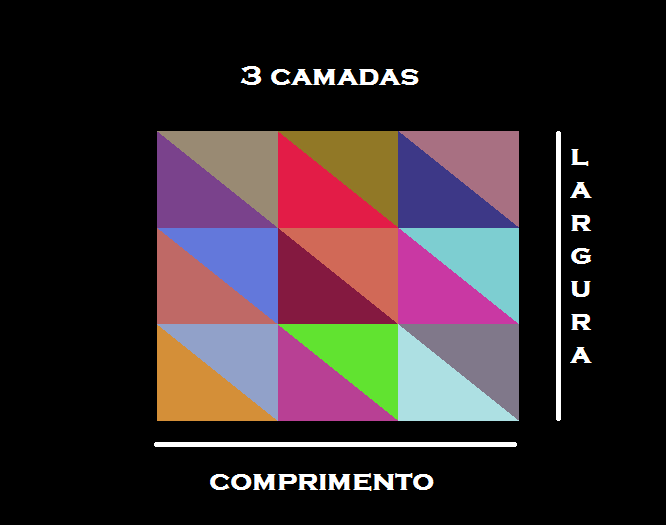
\includegraphics[scale=0.29]{plano.png}
		\caption{Plano com 5 de comprimento, 4 de largura e 3 camadas}
	\end{figure}
	\clearpage
	
	\item[Cubo] \hfill \\
	A função que desenha o cubo recebe como argumento o comprimento do lado e o número de camadas no eixo dos \textit{X} e dos \textit{Z}. Tal como no plano, para centrar o cubo na origem, a variável lado é dividida por dois. Para desenhar esta primitiva, como seria de esperar desenhamos seis faces, e cada uma delas desenhada da mesma maneira que é desenhado um plano.
	
	Optámos por criar um cubo e não um paralelipipedo, pois um paralelipipedo pode ser obtido escalando um cubo.
	
	Visto ser ineficiente, não recorremos à função que cria o plano para construir o cubo (ver secção \ref{evitar mudancas de estado})
	
	\item[Cilindro] \hfill \\
	Este primitiva foi desenhada de um método muito semelhante ao usado no execício da aula prática. A função recebe como argumentos o raio, a altura, o número de camadas verticais e o número de camadas horizontais. Existe uma varíavel \textit{delta} que resulta da operação
	\begin{verbatim}
	float delta = 2 * M_PI / fatias;
	\end{verbatim}
	Ficando guardada nesta variável o ângulo necessário para obter as coordenadas polares. Mais uma vez como a primitiva deve ser desenhada na origem, dividimos a altura por dois. O Cilindro é assim desenhado com recurso a coordenadas polares (ver secção \ref{CoordenadasPolaresEEsfericas}). Posteriormente o cálculo deste ângulo foi modificado para passar a ser calculado a cada iteração para evitar erros de vírgula flutuante (ver secção \ref{Erros de virgula flutuante}).

	\item[Esfera] \hfill \\
	A função que desenha esta primitiva recebe três argumentos: o raio da esfera, o número de camadas verticais e o número de camadas horizontais. É através de dois ângulos e funcões trignométricas que conseguimos desenhar a primitiva. Estas variáveis são:
	\begin{verbatim}
		float alpha = 2 * M_PI / fatias;
		float beta = M_PI / seccoes;
	\end{verbatim}
	Estamos agora a utilizar coordenadas esféricas (ver secção \ref{CoordenadasPolaresEEsfericas}). Existem três ciclos, um que desenha a parte de baixo, outro que desenha a parte de cima e por fim um que desenha as secções intermédias.
	Posteriormente o cálculo destes ângulos foi modificado para passar a ser calculado a cada iteração para evitar erros de vírgula flutuante (ver secção \ref{Erros de virgula flutuante}).
	\begin{figure}[h!b!t!]
		\centering
		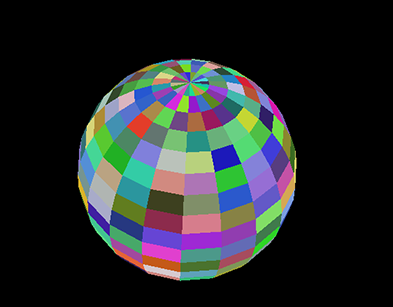
\includegraphics[scale=0.7]{esfera.png}
		\caption{Esfera com 2 de raio, 20 camdas hotizontais e verticais}
	\end{figure}
\end{description}
\clearpage
\subsubsection{Segunda Fase}
Em relação à primeira etapa, nós decimos organizar o nosso trabalho de modo a tornar as coisas mais simples, e para no futuro ser mais fácil a implementação. Para isso foram criadas algumas novas classes.

Criámos uma classe \textbf{CG\_OBJ} que define um \textit{Vertex Buffer Object} (sem índices). De forma simplificada, um \textit{VBO} é buffer onde se guarda um conjunto de vértices correspondente a uma primitiva (ver secção \ref{VBO}).

Para compor vários \textit{VBO} de modo a formar um objecto complexo foi criada a classe \textbf{Figuras}. Esta classe \textit{static} apenas tem um \textit{array} de \textbf{CG\_OBJ} e métodos que compõem elementos desse array para formar figuras complexas. Estes métodos são utilizados pelo \textit{renderScene()} para desenhar objectos construidos por composição de primitivas.

Foram também criadas sub-classes da classe \textbf{CG\_OBJ} correspondentes às várias primitivas: \textbf{Plano}, \textbf{Cubo}, \textbf{Cilindro} e \textbf{Esfera}. De notar que a forma de desenhar as primitivas mudou e, como tal, a nova forma de desenhar primitivas difere consideravelmente da forma que constava na classe \textbf{Primitivas}. Além das quatro primitivas, foi adicionada a classe \textbf{SolidoRevolucao} que foi usada para desenhar copos (ver secção \ref{SolidosRevolucao}).

Também implementámos uma câmara FPS (ver secção \ref{camara fps}) e alterámos a interacção através do teclado com a aplicação (ver \ref{Gestao de input}). De forma a aumentar a escalabilidade do projecto, criámos duas novas classes para o controlo da câmara e teclado. São respectivamente a classe \textbf{Camera} e a classe \textbf{Input}. Ao longo das fases seguintes, ambas as classes \textbf{Camera} e \textbf{Input} foram sofrendo alterações conforme foi necessário.
\newpage
\begin{description}
	\item[Espaço limite do Bar] \hfill \\
	Para simular o espaço do Bar, fizemos com que toda a cena fosse desenhada dentro de um cubo com as seis paredes visíveis.
\begin{figure}[h!b!t!]
	\centering
	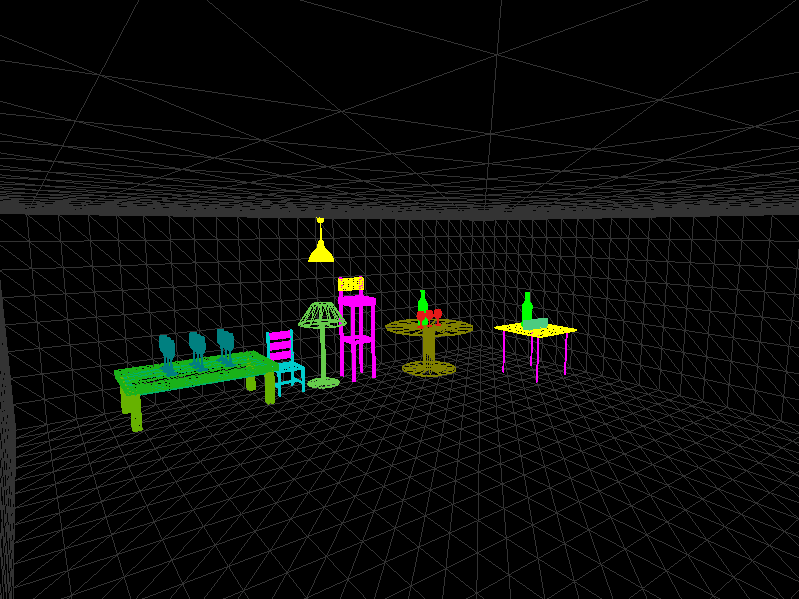
\includegraphics[scale=0.4]{paredes.png}
	\caption{As seis paredes visíveis em modo linha}
\end{figure}
\newpage
\item[Objectos] \hfill \\
Para além do espaço limite do bar, foi também pedido que fossem construídos alguns elementos que se podem encontrar num bar. Estes elementos são desenhados recorrendo aos métodos da classe \textbf{Figuras}.

Para esta fase desenhámos três \textbf{mesas}, sendo que uma delas tem a base e o tampo redondo, outra mesa \textbf{quadrada} e por fim uma mesa \textbf{rectângular} baixa.

A mesa \textbf{quadrada} é a mais simples das três, contendo quatro cilindros que constituem as pernas da mesa e um rectângulo para a superfície.

Temos uma mesa rectangular mais baixa que a quadrada. A mesa é formada por 9 cubos: 4 para as pernas, 4 para o reforço e 1 para a superfície da mesa.

Por fim temos a mesa \textbf{redonda}, que é composta por uma base de suporte inferior e pela superfície superior. A unir estes itens está um cilindro de raio inferior à base e ao tampo. Esta mesa é desenhada com recurso a Sólidos de Revolução (ver secção \ref{SolidosRevolucao}).

Outro elemento do Bar pedido eram as \textbf{cadeiras}, além de cadeiras optámos por também desenhar um \textbf{banco} alto. As pernas, assento e recosto da cadeira são cubos. O banco tem pernas cilíndricas e ambos o recosto e o assento são cubos.
\begin{figure}[h!b!t!]
    \centering
    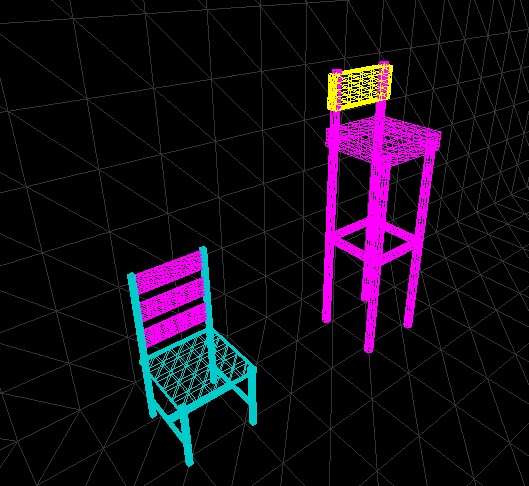
\includegraphics[width=370px, height=340px]{cadeiras.png}
    \caption{Cadeira normal e banco de balcão}
\end{figure}

Apresentamos agora os \textbf{copos} que criámos usando Sólidos de Revolução (ver secção \ref{SolidosRevolucao} para detalhes sobre Sólidos de Revolução). Recorrendo à mesma técnica desenhámos também uma garrafa.
\begin{figure}[!htb]
    \centering
    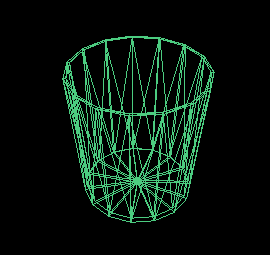
\includegraphics[scale=1]{copo.png}
    \caption{Copo normal}
\end{figure}
\begin{figure}[!htb]
    \centering
    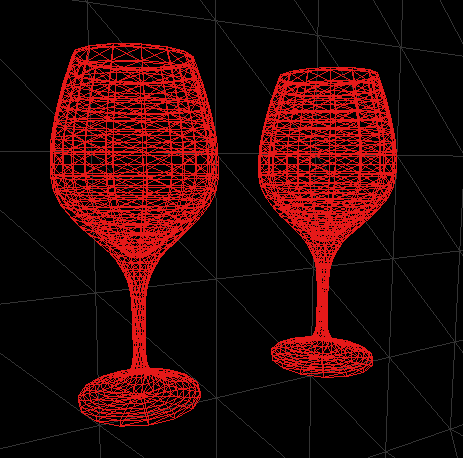
\includegraphics[scale=0.8]{vinho.png}
    \caption{Copo de vinho}
\end{figure}
\begin{figure}[!htb]
    \centering
    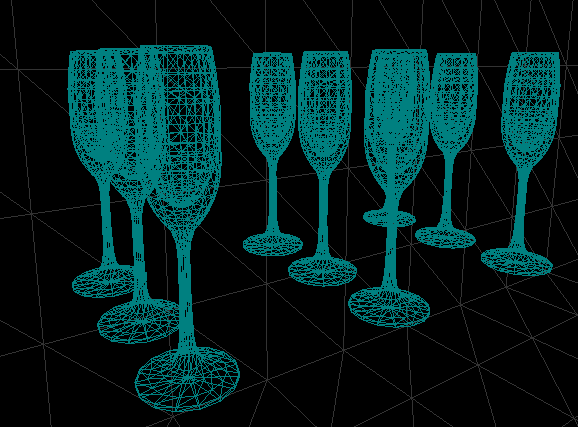
\includegraphics[scale=0.9]{champanhe.png}
    \caption{Copos de champanhe}
\end{figure}
\begin{figure}[!htb]
    \centering
    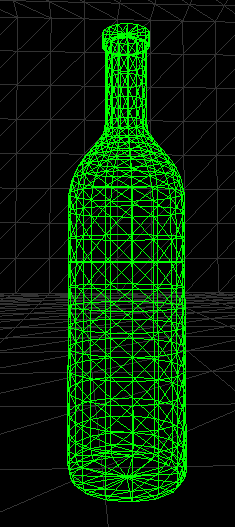
\includegraphics[scale=0.7]{garrafa.png}
    \caption{Garrafa}
\end{figure}

Finalmente o último item pedido eram candeeiros, aqui optámos por fazer dois estilos diferentes, um de tecto e outro de pé. Tanto o candeeiro de tecto e o \textit{abajour} do candeeiro de pé são Sólidos de Revolução. O candeeiro de pé também é formado por uma composição de vários cilindros.
\begin{figure}[!htb]
	\centering
	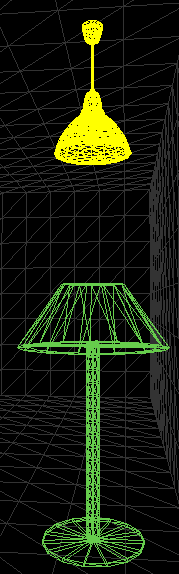
\includegraphics[scale=0.6]{candeeiros.png}
	\caption{Candeeiro de tecto e de chão}
\end{figure}
\end{description}
\clearpage
\subsubsection{Terceira Fase}
Tal como já tinha sido referido anteriormente e no enunciado, um dos objectivos para esta etapa do projecto seria a utilização de \textit{Vertex Buffer Objects} no desenho do Bar. Os \textit{VBO}s que implementámos não são óptimos, pois não utilizam indices. Nesta fase serão implementados \textit{VBO}s com indices (ver secção \ref{VBO}).

\begin{description}
	\item[\textit{VBO}s nas Primitivas] \hfill \\
	Já tinhamos os \textit{VBO}s implementados na segunda fase, portanto nesta fase apenas implementámos indices e adicionámos coordenadas de textura e normais aos vértices.
	
	Nesta fase a classe \textbf{Figuras} continua a ser responsável pela composição de \textbf{CG\_OBJ} em objectos complexos.
	
	\item[Iluminação e Texturas] \hfill \\
	Utilizando as coordenadas de textura e as normais aos vértices nos \textit{VBO}s implementámos texturas e iluminação no nosso Bar. Para não comprometer a escalabilidade do projecto, foram criadas duas novas classes: \textbf{Texturas} e \textbf{Light}. 

\end{description}
\newpage

\begin{figure}[!htb]
    \centering
    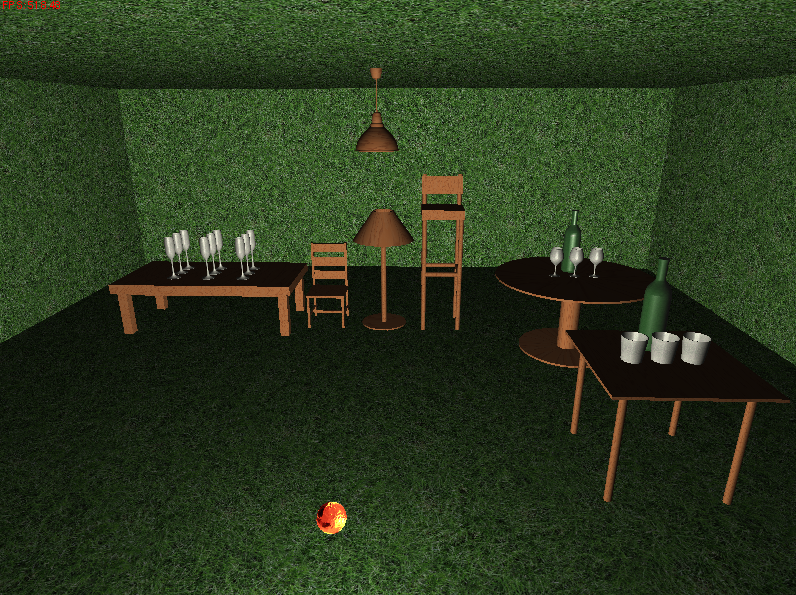
\includegraphics[scale=0.5]{fase3.png}
    \caption{Composição do Bar no fim da fase 3}
\end{figure}

\clearpage
\subsubsection{Quarta Fase}
Nesta fase deve ser apresentado o produto final deste projecto: o Bar. Para esta fase também é pedido que exista iluminação, texturas e uma câmara de movimento livre.

\begin{description}
	\item[Visualização da cena utilizando uma câmara de movimento livre] \hfill \\
	A câmara estilo FPS está implementada desde a segunda fase sob a forma da classe \textbf{Camera}. Esta classe tem sofrido alterações de acordo com as necessidades. Nesta quarta fase a \textbf{Camera} também está encarregue de actualizar os planos do View Frustum (ver secção \ref{view frustum culling} sobre View Frustum Culling).
	
	\item[Utilização de texturas e iluminação] \hfill \\
	As texturas e a iluminação foram implementadas na fase anterior. Nesta fase apenas sofreram alterações para adicionar texturas ou facilitar o uso da classe.
	
	\item[Aplicação com a apresentação da composição geométrica final] \hfill \\
	Depois de compostas as várias primitivas criadas ao longo do projecto, obtemos o produto final: o Bar.

\end{description}
\newpage

\begin{figure}[!htb]
    \centering
    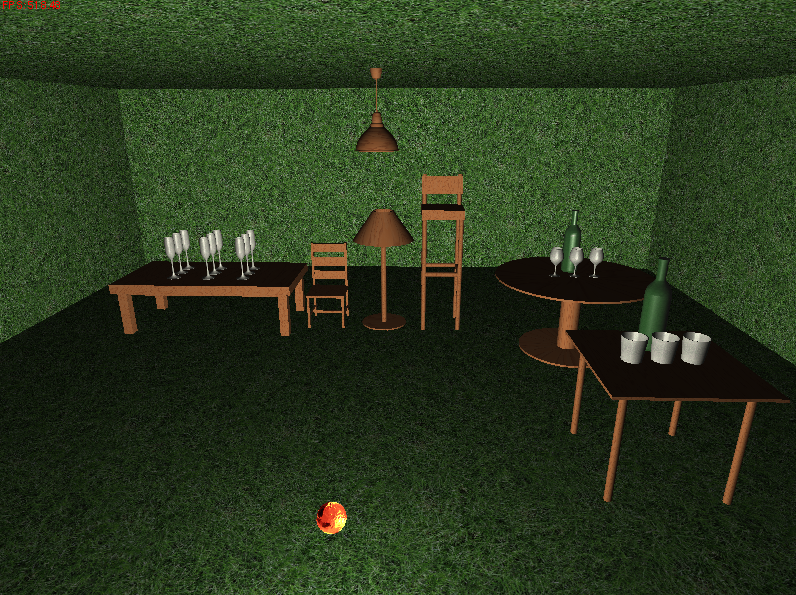
\includegraphics[scale=0.5]{fase3.png}
    \caption{Composição do Bar no fim da fase 3}
\end{figure}

\newpage
\onecolumn
\subsection{Organização do Projecto}
-(DIAGRAMA DE CLASSES IMAGEM)
-um pouco de texto

\newpage
\subsection{Optimização e Técnicas usadas}
Aqui iremos falar das várias técnicas que usamos ao longo do nosso projecto e também de algumas optmizações que fizemos.
\subsubsection{"Camadas" nas primitivas} \label{Camadas nas primitivas}
\subsubsection{Evitar mudanças de estado} \label{evitar mudancas de estado}
\subsubsection{Coordenadas Polares e Esféricas} \label{CoordenadasPolaresEEsfericas}
\subsubsection{Evitar erros de vírgula flutuante} \label{Erros de virgula flutuante}
\subsubsection{Vertex Buffer Objects} \label{VBO}]
nao esquecer a geração dinamica de indices e fazer distinçao entre VBO de fase 2 e 3
\subsubsection{Câmara FPS} \label{camara fps}
\subsubsection{Gestão de input} \label{Gestao de input}
\subsubsection{Sólidos de Revolução} \label{SolidosRevolucao}
\subsubsection{Backface Culling} \label{backfaceCulling}
\subsubsection{View Frustum Culling} \label{view frustum culling}
A implementação do View Frustum Culling permite que não sejam desenhados objectos que não estão no campo de visão da cãmara.
\subsubsection{Bouding Volumes Hierárquicos} \label{bounding volumes hierarquicos}
\subsubsection{Encadeamento de métodos}

\newpage
\section{Navegação e Controlos}
Um dos requisitos finais é a implementação de uma câmara de movimento livre. Nós inicialmente para visualizar as primitivas usavamos menus, em que o utilizador escolhia qual primitiva a visualizar separadamente, em conjunto com outras opções como colorir ou ver em modo de linhas ou todo preenchido. Na segunda fase já podiamos ver uma câmara FPS para ver os objectos construídos, e além disso ainda tinhamos um menu com as opções já atrás referidas. Na terceira fase já ouve alguma evolução na câmara e deixaram de existir os menus. Nesta etapa a câmara é de movimento livre através das teclas do teclado ('w','s','a' e 'd'), e recorrendo à tecla 'z' é possível alternar a visualização para modo preenchido ou só as linhas dos objectos. Com a ajuda da tecla '+' e '-' o utilizador pode aumentar e diminuir a velocidade da câmara. Portanto nesta fase final, a navegação efectua-se recorrendo às teclas 'w', 's' (respectivamente, movimento para a frente para trás) e 'a','d' (movimentação lateral para a esquerda e direita, respectivamente), equanto o rato serve para rodar e controlar o ângulo da câmara. Além disso, como foi feito anteriormente, é possível alternar de estados para preenchido e só linhas, e também aumentar ou diminuir a velocidade da câmara. No canto superior esquerdo, é possível visualizar a quantos FPS está a correr. Nesta fase acrescentamos, além do 'z', o 'x' que activa e desactiva o View Frustum Culling com o primir da tecla.
Todas estas funcionalidades são implementadas nas funções exclusivas do OpenGL para a utilização do rato e teclado. As funções de implementação do teclado e do rato encontram-se no Camara.cpp e Input.cpp.
\clearpage
\section{Conclusão}
Com a chegada do fim deste relatório chegou a altura de se tecerem as conclusões finais.
\newpage




\clearpage
\onecolumn
\section{Fotos}
\begin{center}
    \begin{tabular}{ccc}
        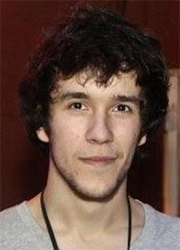
\includegraphics[width=90pt]{bruno.png}&
        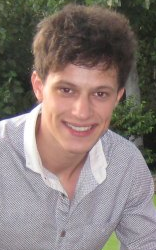
\includegraphics[width=90pt]{serafim.png}\\
        
        \small{\textbf{Bruno Ferreira}}&
        \small{\textbf{Serafim Pinto}}\\
        \small{\textbf{A61055}}&
        \small{\textbf{A61056}}\\
    \end{tabular}
\end{center}
\end{document}